\section{The negative interval unit}\label{sec:negative}

The ordinary interval units have an additional negative-direction analogue
with a sphere incidence condition.  This condition is essential: it is a
degree-two insertion, obtained by allowing the loop in a degree-three
holonomy condition to move through a one-parameter sweep of a sphere.
Throughout this section the determinant transitions on the true ends are
fixed, and all gauge transformations have determinant one.  Sweep
homotopies preserve the chosen sphere orientation.

The proof has four stages: the minimal cap calculation, the comparison
of its two determinant lifts, the chain-map identity, and the
four-step family proving that the map is a unit modulo two.  The local
comparison fixes the weights that will also cancel the spinor lens ends
in Section~\ref{sec:gluing}.

Set
\[
 W'=(-C_2)+C_{-2}\colon Y_2\longrightarrow Y_{-2}.
\]
The capped Seifert classes $F_l,F_r$ are orthogonal, have square $-2$, and
give integral coordinates on $H_2(W';\Z)$.  The two capping disks give an
embedded sphere
\begin{equation}\label{eq:negative:sphere}
 S=F_l-F_r,\qquad S^2=-4.
\end{equation}
The interval of metrics has one endpoint at the primary splitting
$J=Y_\infty=S^3$ and the other at the splitting off
$N'=\nu S$, whose oriented boundary is the corresponding lens space of
order four.  These are the two arc cuts in the polygon construction of
Lemma~\ref{lem:ordinary:polygon}.  Write $t$ for the interval parameter.

Choose an orientation of $S$ and a sweep $\gamma_s$, $0\le s\le1$, from a
constant loop to a constant loop, of degree one onto $S$.  Reparametrize
it to be constant near $s=0,1$.  On the lens collar keep the entire sweep
inside $N'$.  For each $e\in\{0,1\}$ use the determinant
\begin{equation}\label{eq:negative:lifts}
 c_e=e\PD(S),
\end{equation}
with the two determinant bundles identified off $N'$.  Both determinants
have square roots on $W'$: their evaluations on the integral basis
$(F_l,F_r)$ are $(0,0)$ or $(-2,2)$, and $H_1(W';\Z)=0$.
Divide holonomy by the holonomy of that root.  Equivalently, for a sphere
sweep the determinant square root is the one continued from its
collapsed starting loop.  The condition denoted by $x(S)$ is
\begin{equation}\label{eq:negative:cut}
 \Hol_0(a,\gamma_s)=-\id\in\SU(2).
\end{equation}
The target is central, so the condition is independent of the frame
used to record holonomy.  At the collapsed loops the normalized holonomy
is $+\id$, and the condition is absent there, also after a sufficiently
small regularizing perturbation supported away from those endpoints.

The index $i$ is the fixed-limit unframed ASD index of
Section~\ref{sec:ordinary}.  Thus a zero-dimensional count defining the
interval map has
\begin{equation}\label{eq:negative:dimension}
 i+\underbrace{1}_{t}+\underbrace{1}_{s}
       -\underbrace{3}_{\text{holonomy}}=0,
 \qquad i=1.
\end{equation}
Let $B_e$ be this count between the prescribed irreducible generators.
We will specify the relative orientation of its two summands below and
write $B=B_0+B_1$ with those orientations understood.

\begin{theorem}[Negative interval unit]\label{thm:negative:unit}
The counts defining $B$ can be chosen coherently so that
\[
 B\colon C(Y_2;\Z)\longrightarrow C(Y_{-2};\Z)
\]
is an integral chain map.  Its reduction modulo two induces an
isomorphism on Floer homology.  Its integral chain-homotopy class is
unchanged by compatible changes of the interval data and sphere sweep.
The relative sign of the two determinant lifts is local at $N'$,
is independent of the exterior solution, and is preserved under
composition with other cobordisms.
\end{theorem}

We first establish the cap calculation and the signs.  We then compute
the map modulo two by a four-step family.  The analytic inputs are the
ordinary compactness, perturbation, and regular-gluing statements of
Section~\ref{sec:ordinary}, together with the compatible library of
Proposition~\ref{prop:analysis:ordinary-library}.  In the application
below these inputs are used with fixed relative bundle sectors,
product-compatible parameter collars, perturbations independent of
incidence marks, and fixed true-end data.  At a harmonic reducer the
perturbation value is zero and its normal derivative may be varied
equivariantly.  We only glue transverse, isolated matches with no
particle or positive-charge neck loss.  The following dimension and
charge arguments verify those last hypotheses before gluing is used.

\subsection{The minimal cap and relative orientations}

\begin{lemma}[The order-four cap]\label{lem:negative:cap}
Use a determinant square-root normalization on $N'$.  For a fixed
boundary flat $\alpha$, let $h^0(\alpha)$ be the dimension of its parallel
adjoint sections.  The framed cap index and its charge satisfy
\begin{equation}\label{eq:negative:cap-index}
 \delta:=i_{N'}^{\mathrm{fix}}+h^0(\alpha)=8E,
 \qquad
 \begin{cases}
 E\in\Z,&\alpha\text{ central},\\
 E\in\frac14+\Z,&\alpha\text{ trace zero}.
 \end{cases}
\end{equation}
A flat cap misses $x(S)$.  The minimum cap which meets the cut has
$E=1/4$, trace-zero boundary flat, and framed real index two.  With
arbitrarily small compatible equivariant perturbations, its framed
cut-down solutions are harmonic reducible crossings, with signed total
$\pm1$.  Each crossing gives one match with a regular unframed exterior;
there is no additional ordering or framing multiplicity.
\end{lemma}

\begin{proof}
Let $x\in H^2(N';\Z)$ evaluate as one on $S$.  Rationally $x^2=-1/4$.
The normalized boundary representations of its cyclic fundamental group
have generator holonomy $\pm\id$ or a conjugate of
$\diag(i,-i)$.  A reference split connection with summand difference
$d=2x$ has
\[
 E=-\frac{d^2}{4}=\frac14.
\]
With a fixed boundary representative, changing the relative bundle
degree changes $E$ by an integer and the index by eight.  Both central
boundary values have the trivial adjoint boundary correction; the
flat $+\id$ reference has framed index zero.  The trace-zero reference has
framed tangent index zero, since $H^1(N';\R)=0$ and $b^+(N')=0$,
and framed normal complex index one.  Here is the relative calculation
of the latter correction.  Contract the negative section in
$\mathbb F_4$ to obtain $\mathbb P(1,1,4)$.  On their identified smooth
complements the two normal twists agree as complex bundles.  For the
fiber twists of degrees $2,-2$ their Euler characteristics are $3,-1$
on the resolution and $3,0$ on the weighted plane.  Indeed the fiber
line on $\mathbb F_4$ is pulled back from $\mathcal O_{\CP^1}(1)$,
so the two Euler characteristics are $\chi(\mathcal O(2))=3$ and
$\chi(\mathcal O(-2))=-1$.  On the weighted plane with weights
$1,1,4$, the degree-two part has three monomials; the degree-minus-two
part has no sections, no intermediate cohomology, and no top
cohomology, the latter also following from the canonical degree $-6$.
The ASD normal
symbol contributes minus the sum of these characteristics; hence its
relative complex index is
\[
 [-3-(-1)]-[-3-0]=1.
\]
The corresponding flat cone reference has framed index zero.
Excision gives the asserted normal index, and hence
\eqref{eq:negative:cap-index}.  The minimal unframed dimension one is
also the $m=1$ case of the order-four calculation in
\cite[Lemmas~5.2--5.3]{FintushelStern1997}.

The cap is simply connected.  A flat connection after determinant
normalization therefore has trivial holonomy on every loop of the
sweep.  Compactness makes this avoidance persist for sufficiently
small perturbations.  Nonnegative charges in
\eqref{eq:negative:cap-index}, including charges of any neck levels,
then show that the first possible cut cap has $E=1/4$.

At this charge a reducible has unordered difference $\{2x,-2x\}$.
Order the summands by requiring $d(S)=2$.  Their difference restricts
to the degree-two character modulo four, and the ordered normalized
eigenvalue specifies its eigenline at the fixed boundary representative.
Thus ordering does not double the number of connections.  Abelian
Hodge theory supplies a unique ASD extension with these data: existence
uses the vanishing of the self-dual obstruction, while the difference
of two such solutions has exact curvature, zero $L^2$ curvature norm
by integration by parts, and then is gauge trivial because $H^1(N')=0$.

The normalized chosen eigenline has degree $d(S)/2=1$.  If $D_s$ is
the part of the swept sphere preceding $\gamma_s$, its holonomy is
\[
 \lambda(s)=\exp\left(2\pi i\int_{D_s}F_{\mathrm{eig}}/(2\pi i)\right).
\]
The continuous real phase changes by one from one collapsed loop to
the other.  Consequently $\lambda$ has winding one, up to reversal of
the sphere orientation.  Its transverse crossings of $-1$ have signed
sum $\pm1$.  Both eigenvalues equal $-1$ at such a crossing; they
describe a single instance of \eqref{eq:negative:cut}.

For completeness, regularity here concerns the \emph{framed} cap.
Its tangent operator is already regular of real index zero.  The
normal operator is complex linear of index one.  Holonomy derivatives
detect its kernel modulo infinitesimal gauge: if every based-loop
variation is a simultaneous infinitesimal conjugation, transport from
the base point constructs that gauge; its off-diagonal part decays
because the trace-zero boundary flat has no off-diagonal parallel
sections.  A finite collection detects the finite-dimensional kernel.
In a slice fixing the boundary torus, torus-equivariant linear outputs
in these detected directions prescribe kernel-to-cokernel variations.
These outputs vanish on commuting data.  They therefore make the
complex operator surjective without moving the harmonic solution.
After this step its normal kernel has complex dimension one.

The holonomy target tangent at $-\id$ is the direct sum of a real toral
line and an off-diagonal complex line.  Vary the cut so that the mark
derivative is nonzero in the toral line at every crossing, and its
derivative on the normal kernel is a complex isomorphism onto the
off-diagonal line.  These variations are allowed by the same sample
slice construction.  The resulting dimension is
\begin{equation}\label{eq:negative:framed-cut}
 \underbrace{2}_{\text{framed cap index}}
 +\underbrace{1}_{\text{mark}}-3=0.
\end{equation}
The off-diagonal isomorphism is complex oriented, so the remaining
crossing sign is precisely the toral winding sign.  This proves the
signed count assertion.

An irreducible cap satisfying the cut would have a positive-dimensional
orbit under the residual framing torus $H=\U(1)$.  Equivariant
transversality would make the framed cut locus zero-dimensional, so
such a solution is absent.  A reducible crossing is fixed by $H$:
its parallel stabilizer absorbs that action.  Accordingly one can
glue the framed cap to the unframed exterior, or equivalently divide
two framed matching spaces by the diagonal $H$; either convention
gives exactly one match per crossing.  At the minimum there is no
positive cap or neck charge available, and a flat cap misses the cut,
so there is no further end of this local count.  These regularity
choices are required only at the finitely many transverse exterior
parameter values; they can be localized, extended over parameter
collars, and copied by tensoring to the second lift.
\end{proof}

\begin{proposition}[Local relative signs]\label{prop:negative:local-sign}
There is a relative orientation convention for the two lifts in
\eqref{eq:negative:lifts} under which their minimal lens ends cancel
over $\Z$.  The comparison uses identical exterior data, including
relative bundle degree, and is independent of the exterior field.
It commutes with gluing on other seams and is multiplicative for
disjoint sphere caps.  Adding a coupled complex Dirac determinant
preserves this convention.
\end{proposition}

\begin{proof}
Fix coherent Floer orientations for the unflipped sector.  Fix also a
representative $\alpha$ of the trace-zero lens flat, and realize the
two framed relative cap sectors at charge $1/4$.  On the cap,
$\PD(S)=-4x$, so tensoring by a line of first Chern class $a=-2x$
changes the determinant by $2a=\PD(S)$.  Starting with $c(S)=0$,
the relative Chern numbers change by
\begin{equation}\label{eq:negative:tensor-charge}
 \Delta c^2=-4,\qquad \Delta c_2=-1,\qquad
 \Delta\left(c_2-\frac{c^2}{4}\right)=0.
\end{equation}
Here $\alpha$ is recorded in the fixed common exterior determinant
normalization.  The twisting line has the order-two flat character
on the boundary in that convention.
It carries $\diag(i,-i)$ to $\diag(-i,i)$, which is conjugate back
to $\alpha$.  Choose a determinant-preserving parallel boundary
identification making that conjugation.  Its remaining ambiguity is
the connected centralizer, and does not reverse an orientation.
Equality of the trace-free charges with this boundary identification
fixes the relative $c_2$ change in \eqref{eq:negative:tensor-charge}.
Thus gluing this tensor cap to the unchanged exterior gives precisely
the flipped bundle, with unchanged relative degree outside the cap.

Here is the determinant-line comparison, including its relation to any
previous choice of orientations for the individual sectors.  Write
\[
 K_e=\det D_{N',e}^{\mathrm{fr}}\otimes\det\R_s
          \otimes\bigl(\det\mathfrak{su}(2)\bigr)^*
\]
for the framed cap line with its mark and cut factors, and let
$\lambda_V$ include the common unframed exterior and its remaining
parameter and cut factors.  With their fixed ordering, determinant
gluing gives maps $\Gamma_e:\lambda_V\otimes K_e\longrightarrow
\lambda_e$ to the full constrained orientation lines.  Tensoring and
the chosen boundary conjugation compare the full cap deformation and
cut complexes and give $\tau_{\mathrm{cap}}:K_0\longrightarrow K_1$.
Set
\begin{equation}\label{eq:negative:orientation-comparison}
 \Phi=\Gamma_1\circ(\id\otimes\tau_{\mathrm{cap}})
                 \circ\Gamma_0^{-1}.
\end{equation}
For conventional sector orientations $o_e$, define $s\in\{1,-1\}$
by $\Phi(o_0)=s\,o_1$.  Choose weights according to
\begin{equation}\label{eq:negative:lift-weights}
 \varepsilon_1=-s\varepsilon_0,
 \qquad
 \Phi(\varepsilon_0o_0)=-\varepsilon_1o_1.
\end{equation}
This is exactly the opposite count orientation required for paired
crossings.  It neither assumes nor needs $s=1$.  In particular a Weyl
boundary conjugation can reverse an ordered toral generator and
conjugate an ordered off-diagonal complex coordinate; all such signs,
including the framing and target factors, are part of
$\tau_{\mathrm{cap}}$.

Take tensor-related equation and cut data and tensor-related roots:
a root after tensoring is the old root tensored with the twisting
line.  These are the intrinsic cap roots continued from the collapsed
loop; their boundary identifications need not coincide with the fixed
common exterior normalization used to record $\alpha$.  Thus the
boundary value changes from $\alpha$ to $-\alpha$ in the latter
convention, whereas normalized sweep holonomy is unchanged before the boundary
conjugation.  Conjugation preserves the central target $-\id$ and its
orientation in $\SU(2)$.  Thus the matched cut points correspond and
\eqref{eq:negative:lift-weights} makes their contributions opposite.
The weights may equivalently be absorbed into the orientations of
$B_e$.  In later compositions they give a weighted sum of the ordinary
sector counts.  The canonically oriented cap pairing used for
nonvanishing is left unchanged: the subsequent repetition argument
uses this signed map $B$, whose reduction modulo two is independent
of the weights.  No equality with an unweighted sum of Donaldson
invariants on the assembled manifold is required.

We explain why the convention extends consistently away from the wall.
The integral-lift ASD determinant line with chosen true-end orientations
is orientable on the \emph{determinant-one gauge quotient}, as fixed in
Convention~\ref{conv:ordinary:index}.  Its orientation double cover
therefore has trivial monodromy, including around a path closed by a
gauge transformation.  The reference connection spaces with the
specified collar representative and relative degree are affine and
connected, so their quotients are connected.  Connectedness permits
transport from the chosen reference; quotient orientability makes that
transport independent of the path.  This extends the comparison
\eqref{eq:negative:orientation-comparison} as a comparison of
orientation torsors with one constant relative sign.

In choosing $\alpha$, fix its internal framing degree so that the cap
sector has charge $1/4$.  An integral gauge degree changes this relative
charge by the same integer.  Hence a boundary gauge relating two actual
minimum-charge walls in this sector has degree zero.  In the fixed
boundary trivialization its homotopy class lies in
$[\partial N',\SU(2)]\cong H^3(\partial N';\Z)\cong\Z$, classified
by that degree.  A degree-zero gauge is nullhomotopic; use a nullhomotopy
on the collar and the identity beyond it to extend it over the cap.
Nonzero degree would change the prescribed relative sector.  The
remaining parallel ambiguity in the boundary conjugation lies in the
connected torus stabilizer and extends as a parallel cap gauge.  There
is consequently no additional boundary-gauge sign in the comparison.
Interpolations here take place in connection space; no path of
solutions is asserted.

Associativity of determinant-line gluing now proves naturality under
adding an exterior cylinder or cobordism: in either gluing order the
same cap reference and the identity on the same exterior are used.
The two raw framed cap indices are the same even number, namely two,
and the two constrained indices in \eqref{eq:negative:framed-cut} are
zero.  With one fixed ordering of cuts and parameters there is no
exterior-dependent interchange sign.  Comparisons on disjoint caps
therefore multiply.  Finally a coupled Dirac determinant has its
complex orientation, and tensoring and the boundary conjugation act
complex linearly on that factor.  It introduces no new relative sign.
\end{proof}

The square roots used to normalize holonomy do not identify the two
global relative bundles with their fixed exterior and true-end data.
In particular a root of their determinant difference need not be
trivial on that exterior.  The comparison just proved is the localized
cap replacement with its boundary conjugation.  The same comparison
will be used for the coupled regular cap in
Proposition~\ref{prop:gluing:regular-cap}.

\subsection{The chain map and its invariance}

\begin{proposition}[Chain property and invariance]\label{prop:negative:invariance}
With the signs of Proposition~\ref{prop:negative:local-sign}, $B$ is
an integral chain map.  Compatible homotopies of equation data and
incidence representatives give integral chain homotopies.  The allowed
representative homotopies include smooth conjugation-equivariant
homotopies of the normalized based holonomy paths, relative to their
collapsed endpoints, under the following requirements.  Their exact
compact supports remain in the specified parts, they persist under
ideal convergence away from a support hit, and the equation data do
not depend on the incidence mark.  At the lens endpoint the test is
supported in $N'$, its two lifts are tensor-paired with the same
exterior, and its flat-cap and collapsed-endpoint avoidance holds
throughout.  The data admit regularization preserving these
requirements.  The homotopy of the incidence representative need not
be small.  Near the primary $J$ endpoint the unconstrained equation
exclusion requires no additional behavior of the representative.
\end{proposition}

\begin{proof}
The boundary relation for the count \eqref{eq:negative:dimension} uses
$i=2$.  At $J$, with no remaining interval parameter, a central contact
costs at least three by Lemma~\ref{lem:ordinary:central-cost} and
$b^+(W')=0$.  This excludes the face even if the incidence condition
is discarded.  At a true central end without the $J$ cut the same
cost is accompanied by a nonconstant irreducible trajectory towards
the prescribed generator.  That trajectory costs at least one more
index, giving $4-1>2$ even after the interval parameter is allowed.
A bubble costs eight index before its four position parameters;
even discarding the degree-two insertion leaves too much codimension
in these zero- and one-dimensional families.  Equivalently, project
to the remaining equation solution before introducing the incidence
mark: its index has decreased by eight and it has at most one
equation parameter.  It is excluded by ordinary regularity and the
same reducible-group estimate.

At the lens endpoint a flat cap misses the cut.  Thus
Lemma~\ref{lem:negative:cap} gives $\delta\ge2$, with neck charge
included.  The exterior is measured after a reference filling by the
cap; it has $b^+=0$ and no equation parameters.  For a central outer
limit the reducible estimate remains
$8E_{\mathrm{ext}}-3(1+b^+_{\mathrm{filled}})$: excision subtracts
exactly the cap contribution $\delta$, so no boundary correction is
lost.  Reducible groups and forbidden central contacts are consequently
excluded as above.  Regular irreducible exteriors have nonnegative
index.  The only lens boundary with $i\le2$ is therefore
\[
 i=2,\qquad \delta=2,\qquad i_{\mathrm{ext}}=0.
\]
It consists of an isolated regular irreducible exterior and a minimal
cut cap, without further breaking.  Lemma~\ref{lem:ordinary:regular-gluing}
applies: the framed cap is regular and absorbs the boundary stabilizer,
and all matching and cut derivatives are transverse.  It gives exactly
the end counted by Lemma~\ref{lem:negative:cap}.  The two lifts cancel
by Proposition~\ref{prop:negative:local-sign}.

All remaining ends are the ordinary irreducible trajectory breaks at
the true ends.  Their oriented boundary formula is precisely the
chain-map equation for $B$ (with the usual degree convention).
For a homotopy allow one additional common family parameter, so that
at most two parameters enter the equation data, independently of the
incidence mark.  Its chain-homotopy count has index zero and its boundary
relation index one.  At the
primary face the estimate is $3-1>1$; at a true central contact it is
$4-2>1$.  Lens boundaries, when present, are the same paired minimal
caps with their common exterior.  Bubbling is again excluded after
dropping the insertion.  These are all faces of the parameterized
compactification.  The oriented boundary formula supplies the desired
chain homotopy.  These arguments use smallness of the equation
perturbations for the energy exclusions, but no smallness of the
incidence-representative homotopy: its relative endpoint condition and
flat avoidance exclude mark endpoints and zero-charge lens caps,
its support and persistence hypotheses identify the ideal limits, and
its tensor pairing gives the same lens cancellation.  In particular
sweeps may be transported along collars or changed near $J$, where
the exclusion did not use the test.

To check explicitly that such a homotopy preserves the insertion,
work first in a framed configuration slice.  Its evaluation maps
are a homotopy
\[
 F_h:\mathcal B\times([0,1],\{0,1\})
           \longrightarrow(\SU(2),\{\id\}),\qquad 0\le h\le1.
\]
Pulling back the oriented degree-three class of the central incidence
condition and integrating over the mark gives its degree-two
transgression.  A homotopy relative to the mark endpoints preserves
this class.  The construction descends from framed slices because
the homotopy is conjugation-equivariant and conjugation preserves the
target orientation.  Its regular parameterized incidence cobordism
is exactly the one used in the boundary argument above.
\end{proof}

We turn to the mod-two computation.  Consider the four-step path
\begin{equation}\label{eq:negative:four-step}
 2\longrightarrow\infty\longrightarrow0
     \longrightarrow\infty\longrightarrow-2
\end{equation}
on a cobordism $W$.  Its three-dimensional associahedral family has
nine facets: the three primary cuts $Z_1,Z_2,Z_3$ and the six cap cuts
$M_{02},M_{03},M_{04},M_{13},M_{14},M_{24}$.  A facet carries the
product of the remaining parameter families, as in
Lemma~\ref{lem:ordinary:metric-families}.

\subsection{The four-step family and its boundary faces}

\begin{lemma}[Topology and determinant sectors of the four-step family]
\label{lem:negative:four-topology}
The group $H_2(W;\Z)$ has integral coordinates $F_l,F_r,A,U$, with
$F_l^2=F_r^2=-2$, an orthogonal hyperbolic pair
$A^2=U^2=0$, $A\cdot U=1$, and $F_l,F_r$ orthogonal to that pair.
Moreover $H_1(W;\Z)=0$ and $b^+(W)=1$.  The interior side spheres are
\[
 S_l=A-F_l,\qquad U,\qquad S_r=A-F_r,
\]
and form the chain with weights $[-2,0,-2]$.  For
\begin{equation}\label{eq:negative:four-determinants}
 c=\PD(U)+e\PD(S_l)+e'\PD(S_r),\qquad e,e'\in\{0,1\},
\end{equation}
the face at $Z_2$ is the product of the two ordinary interval units
of Theorem~\ref{thm:ordinary:units}.
\end{lemma}

\begin{proof}
The two outside traces split off across $S^3$ and give $F_l,F_r$.
The doubled zero-trace portion is represented by a zero-framed knot
handle and a linked meridian handle.  The latter gives the square-zero
sphere $U$ and the capped Seifert surface gives its primitive dual
$A$.  Their linking number is one; the two zero framings give their
self-intersections zero.  This is an integral handle basis, and the
meridian normally generates the relevant fundamental group, so the
displayed homology and positive rank follow.  The common capped
surface can also be represented on $Z_2=Y_0$ and pushed to either
side of the middle cut.  Subtracting its capping disk on the outside
trace gives $S_l,S_r$, with intersections exactly as stated.

On the left half of $Z_2$, $\PD(U)$ evaluates as $(0,1)$ on
$(F_l,A)$; on the right it evaluates as $(1,0)$ on $(A,F_r)$.
The two additions in \eqref{eq:negative:four-determinants} are supported
in their respective halves.  Thus the determinant transition at $Z_2$
can be chosen common to all four sectors.  The resulting restrictions
are those of $g_+:Y_2\to Y_0$ and its negative-side counterpart
$g_-:Y_0\to Y_{-2}$.  Each has index $-1$ with one parameter;
their product face has index $-2$ with two parameters and induces a
mod-two isomorphism.  A fixed tensor or endpoint identification in
this description only composes it with a Floer automorphism.
\end{proof}

\begin{lemma}[The other associahedron facets]\label{lem:negative:faces}
In the boundary relation at index $i=-2$ for the family
\eqref{eq:negative:four-step}, the $M_{04},M_{03},M_{14},Z_1,Z_3$
facets and all their degenerations contribute nothing.  The
$M_{02},M_{24}$ contributions cancel modulo two by their respective
determinant flips.  The remaining terms are the product at $Z_2$,
the face $M_{13}$, and ordinary true-end breaks.
\end{lemma}

\begin{proof}
At $M_{04}$ the enclosed chain has intersection matrix
\[
 Q=\begin{pmatrix}-2&1&0\\1&0&1\\0&1&-2\end{pmatrix},
 \qquad
 Q^{-1}=\begin{pmatrix}-\tfrac14&\tfrac12&\tfrac14\\
 \tfrac12&1&\tfrac12\\\tfrac14&\tfrac12&-\tfrac14\end{pmatrix}.
\]
Replacing its middle zero-sphere cap by $D=S^1\times D^3$ joins the
two $\infty$ sides, leaving exactly $N'$.  This identifies their
oriented links.  The determinant evaluation vector is
$Q(e,1,e')^t$, so its restriction to that link is trivializable.
Every boundary eigenline extends over the chain, because the
restriction from its integral cohomology onto the lens cohomology is
surjective.  A split reference with difference evaluations
$(d_l,b,d_r)$ has
\begin{equation}\label{eq:negative:chain-square}
 d^2=-\frac{(d_l-d_r)^2}{4}+b(d_l+d_r)+b^2.
\end{equation}
Here $d_l,d_r$ are odd, since
$c(S_l)=1-2e$ and $c(S_r)=1-2e'$.  Hence the square is integral and
$E\in\frac14\Z$.  Charge zero is impossible, even at a corner:
nonnegative charges on all cap pieces and levels would make all of
them flat; their matching would give a flat adjoint cap, whereas its
restriction to an outside sphere has nonzero $w_2$.  Thus $E\ge1/4$.

Compared with $N'$, this cap has Euler characteristic greater by two
and the same signature.  The excision formula therefore gives its
framed contribution, including the matching correction, as
\begin{equation}\label{eq:negative:large-shift}
 8E-3\ge-1.
\end{equation}
The exterior has no parameters and has $b^+=0$ after virtual $N'$
filling.  The central-group estimate, including any true-end
trajectories, and irreducible regularity give exterior index at least
zero.  The sum is greater than $-2$, excluding $M_{04}$.

For $M_{03}$ the chain is $[-2,0]$, and the reversed chain occurs at
$M_{14}$.  The inverse intersection matrix gives
\[
 d^2=2b(d+b).
\]
Its outside evaluation $d$ is odd; $b$ and $d+b$ have opposite
parities, so $d^2$ is divisible by four.  The cap charge is a positive
integer.  Positivity follows by the same odd-sphere flat obstruction,
including at broken corners.  Comparison with a ball gives shift
$8E-3\ge5$.  The virtually filled exterior has $b^+=0$.
Even allowing all remaining parameters on its irreducible components
cannot reduce this contribution to index $-2$.  These facets are
therefore absent as well.

The small caps $M_{02},M_{24}$ are the odd-determinant $-2$ disk
bundles of Section~\ref{sec:ordinary}.  Their trace minimum has charge
$1/8$ and framed shift zero relative to its reference filling.
Nonminimum charge has strictly larger shift.  At a minimum a single
harmonic reducer gives the framed regular match, and the flip supported
on that sphere gives a second copy with the same exterior.  The two
copies cancel modulo two.  To justify applying this local description,
we check that no exceptional exterior or corner can intervene.

Away from the larger cap facets already excluded, fill back any small
odd cap by its reference.  The sum of positive ranks of the primary
pieces is at most one.  A maximal reducible group contributes at least
$3(1-b^+_{\mathrm{group}})$, including its two exterior matches, by
Lemma~\ref{lem:ordinary:central-cost}.  If there is no primary cut,
a group using the positive rank must contain the whole main cobordism
and needs two nonconstant trajectories to the prescribed irreducible
ends.  If there is one primary cut, such a group touches an end and
needs at least one trajectory; with at most $p=2$ remaining parameters
its lower bound is $1-p\ge-1>-2$.  At two or more primary cuts at most
one parameter remains, and the group bound alone is greater than
$-2$.  A central contact with no such group costs at least three
before parameter subtraction.  Nonminimum small caps and bubbles
increase these bounds.  Consequently the only small-cap matches are
minimum caps with exteriors that are irreducible and rigid in their
remaining parameters, away from the corners.

The primary cuts $Z_1,Z_3$ are on $S^3$, which has no irreducible
Floer generators.  Any prospective contact there is one of the
forbidden central configurations just excluded.  The only surviving
primary facet is $Z_2$, the product in
Lemma~\ref{lem:negative:four-topology}.  The nine-facet list is now
exhausted except for $M_{13}$.  Ordinary irreducible breaking at the
two true ends supplies the differential terms in the family homotopy
relation.
\end{proof}

The remaining facet $P=M_{13}$ is a pentagon.  It separates
$N_U=\nu U\cong S^2\times D^2$ from $V=W\setminus N_U^\circ$ and
has link $L=S^1\times S^2$.  Its five edges are
\begin{equation}\label{eq:negative:pentagon-edges}
 Z_1,\ Z_3,\ M_{03},\ M_{14},\ M_{04}.
\end{equation}
In particular it meets neither small flip facet.

\subsection{The selected center and the interval count}

The remaining task is to turn the pentagon count into the interval count
that defines $B$.  We first identify the flat on $L$ selected by a flat
$N_U$.  Replacing $N_U$ by $D=S^1\times D^3$ will then express this
matching as a loop-holonomy condition.  The final step contracts the loop
through two disks whose union represents $\pm S$, producing the
degree-two sphere test.

\begin{lemma}[The root mismatch and the selected center]
\label{lem:negative:root}
Only the sectors $e=e'$ have a flat limit at $L$.  After a tensor
identification fixed on the true ends, their determinants are
\begin{equation}\label{eq:negative:surviving-determinant}
 \PD(U)+e\PD(F_l-F_r),\qquad e=0,1.
\end{equation}
Replacing $N_U$ by $D=S^1\times D^3$ gives $W'$ with determinant
$e\PD(S)$.  If the exterior is normalized using a square root from
$W'$, a flat $N_U$ matches it exactly when the normalized holonomy
of the generator of $\pi_1(L)$ is $-\id$.
\end{lemma}

\begin{proof}
The determinant evaluates on $U$ as $e+e'$.  A projectively flat
connection on $S^1\times S^2$ has trivial $w_2$ on its $S^2$, since
its representation factors through the circle.  Thus $e\ne e'$
is impossible.  In the $e=e'=1$ sector tensor by the line of class
$-\PD(S_l)$, canonically trivial off that sphere.  This changes the
determinant by $-2\PD(S_l)$ and gives
\[
 \PD(U)-\PD(S_l)+\PD(S_r)
   =\PD(U)+\PD(F_l-F_r).
\]
It proves \eqref{eq:negative:surviving-determinant}; the $e=0$ sector
requires no tensoring.  The class $\PD(U)$ can be represented inside
$N_U$, while the second term survives the replacement.  The polygon
replacement joins the identical $\infty$ sides and yields $W'$,
including its fixed true-end identifications.

There are square roots of the determinant separately on $N_U$ and on
$V$: use the root on $W'$ for $V$.  Their root structures on $L$
differ by a flat sign line $Q\in H^1(L;\Z/2)$.  The Mayer--Vietoris
connecting homomorphism sends $Q$ to the obstruction $c\bmod2$ to
a square root on $W$.  This obstruction is nonzero, since
\[
 c(A)=U\cdot A+e(F_l-F_r)\cdot A=1.
\]
Equivalently, if the root structures matched they would glue to a
global root, contradicting this odd evaluation.  As
$H^1(L;\Z/2)=\Z/2$, $Q$ is its nontrivial character and is $-1$
on the circle generator.  A normalized flat connection on the simply
connected cap $N_U$ has generator holonomy $+\id$.  Changing from
its root to the exterior root multiplies that holonomy by $Q$, giving
$-\id$.  Conversely this sign change makes any exterior limit at
$-\id$ agree with the flat cap.  This establishes the selected center
and not merely its image in the projective flat space.
\end{proof}

\begin{lemma}[The surviving pentagon count]\label{lem:negative:pentagon}
At index $i_{\mathrm{total}}=-2$ the face $P$ consists of isolated
regular exterior matches at the selected center with a flat $N_U$.
Their count induces a mod-two isomorphism.  It is also the count on
$W'$ over $P$ at index $i'=1$, with the degree-three condition
\begin{equation}\label{eq:negative:beta-cut}
 \Hol_0(a,\beta)=-\id,
 \qquad \beta=S^1\times\{0\}\subset D,
\end{equation}
when the $D$--exterior neck is sufficiently long and finite.
\end{lemma}

\begin{proof}
Leave $N_U$ unperturbed at this cut.  Relative to a virtual flat
$D$ filling, index excision gives
\begin{equation}\label{eq:negative:zero-replacement-index}
 i_{\mathrm{filled}}
   =i_V^{\mathrm{fix}}+h^1
   =i_{\mathrm{total}}+3-8E_{N_U}\le1,
 \qquad E_{N_U}\in\Z_{\ge0}.
\end{equation}
Any nonflat hard-neck level is included in $E_{N_U}$.  The charge is
integral because the Chern--Simons value is constant on this flat
space and the cap has a zero-charge reference.  The filled exterior
has $b^+=0$ and at most two equation parameters.  If $E_{N_U}\ge1$,
then $i_{\mathrm{filled}}\le-7$, which is incompatible with
irreducible regularity or the central-group lower bound.  Positive
neck or cap charge is therefore impossible.  An additional primary
$S^3$ cut leaves at most one parameter, and costs three.  A forbidden
true central contact also needs an extra irreducible trajectory and
costs at least $4-p>1$ for $p\le2$.  The larger cap corners have
already been excluded in Lemma~\ref{lem:negative:faces}.

At the selected center $h^0=h^1=3$.  Varying the flat in a framed
slice uses three real parameters; imposing the center removes all
three.  It is not a codimension-one endpoint condition on the
conjugacy interval.  The dimension of a prospective exterior match is
\[
 i_{\mathrm{filled}}+p-3\le1+2-3=0.
\]
It can be nonnegative only at $E_{N_U}=0$, $p=2$, and
$i_{\mathrm{total}}=-2$, and is then zero.  Generic compatible
exterior data give transverse matches.

The flat $N_U$ is regular when the boundary flat is allowed to vary
before matching.  Its framed fixed-limit infinitesimal kernel is
zero, since $H^1(N_U)=0$; the three boundary flux obstructions in
the self-dual equation are killed by the three flat parameters,
componentwise by the Abelian relative Hodge exact sequence.  Its full
parallel group absorbs the matching rotations.  Thus this is an
isolated regular matched problem of exactly the type in
Lemma~\ref{lem:ordinary:regular-gluing}, with coefficient one.
The associahedron boundary relation, using
Lemma~\ref{lem:negative:faces}, identifies its map on homology with
the unit at $Z_2$.  This proves the first assertion.

For the second assertion replace $N_U$ by $D$ and retain the same
limiting exterior.  The index becomes $i'=1$.  The framed flat
family on $D$ is locally the three-dimensional group of generator
holonomies near $-\id$; its evaluation on $\beta$ is the identity.
Consequently \eqref{eq:negative:beta-cut} regularly fixes that flat,
and $i'+2-3=0$.  A nonflat $D$ component or hard-neck loss costs
a positive integer charge and is excluded by the same filled-exterior
estimate.  Regular gluing therefore gives exactly the previous
center matches at every sufficiently long finite neck.

Here is the required uniform boundary check.  Keep the exterior of
$M_{04}$ fixed and common for the two sectors, independent of its
cap parameters; both flip spheres are inside that cap.  After
replacement denote the corresponding edges by primes.  The
$Z_1,Z_3$ edges still cut on $S^3$ and are excluded with $p\le1$
even without \eqref{eq:negative:beta-cut}.  The cap at $M_{04}'$
is $N'$; a nonflat contribution has framed shift at least two and
the exterior has no parameters, so it cannot occur at $i'=1$.
At $M_{03}',M_{14}'$ the caps are balls and a nonflat contribution
has shift at least eight.  On these three edges the zero-charge
caps in the filled manifold are simply connected and contain $\beta$;
their normalized flat holonomy is $+\id$, so they miss the cut.
The same assertion holds if the long $D$ neck breaks simultaneously:
its matching zero-charge fields glue to a flat on the same simply
connected filled cap.  The normal-gap estimate and controlled
harmonic drift of Lemma~\ref{lem:ordinary:neck-decay} show that a
loop in a middle slice sees that same flat orbit.  This rules out
escape down the long neck and proves exhaustion, including the
compatible corners.  The true-end determinant identifications remain
fixed throughout the tensor and replacement operation.
\end{proof}

\begin{lemma}[Contraction of the pentagon to the interval]
\label{lem:negative:sweeps}
The map on homology counted in Lemma~\ref{lem:negative:pentagon}
agrees modulo two with $B$.
\end{lemma}

\begin{proof}
We describe the contraction disks, since their location determines
which boundary avoidances remain valid.  In the polygon after the
$U$ replacement, let $E=[a,b]$ be the merged $\infty$ side.  Its
preimage is
\[
 \bigl([a,b]\times S^1\bigr)
  /\bigl(\{a\}\times S^1\text{ and }\{b\}\times S^1
       \text{ collapsed separately}\bigr),
\]
an embedded sphere.  Let $[u,v]\subset(a,b)$ be the inserted $D$
portion and choose $u<t_0<v$.  The surviving circle over $t_0$
is $\beta$.  The preimages of
$[a,t_0]$ and $[t_0,b]$ are disks $\Delta_l,\Delta_r$ with common
boundary $\beta$.  Their union is the merged side sphere.  Before
replacement its class is, up to orientation, $S_l-S_r$; hence after
replacement it is $\pm(F_l-F_r)=\pm S$.

The $M_{04}'$ arc encloses the entire merged side and contains both
disks.  The $M_{03}'$ arc can end on the merged side at a point
$t_+>v$, so its one-corner cap contains $\Delta_l$ and all of $D$;
the $M_{14}'$ arc can end at $t_-<u$, and its cap contains
$\Delta_r$ and all of $D$.  These choices come from nesting the
original $N_U$ cut inside the respective larger cap.  The two-disk
chart at the unique basis corner identifies each one-corner cap
with a ball.  These two ball cuts are incompatible facets and are
never imposed simultaneously.  At a corner with $M_{04}'$, the
appropriate one-corner cap is nested in that outer cap.  Slight
collar displacements put the disks in the required interiors without
altering their boundary or their union class.

Choose an embedded interval $I\subset P$ from the interior of
$M_{04}'$ to a primary $Z$ edge, separating $M_{03}'$ from
$M_{14}'$, as in Figure~\ref{fig:negative:contraction}.
It divides $P$ into two regions.  On the first region
contract $\beta$ through $\Delta_l$, and on the second contract it
through $\Delta_r$.  Denote the contraction parameter by $s$.
Transport the contractions over the parameter collars so that, at
each cap edge, the loops remain in the disk just specified.  The
metrics and ASD perturbations have the two parameters of $P$ and
are independent of $s$.  At $s=0$ we recover the original
degree-three condition; at $s=1$ the loop is collapsed and misses
$-\id$.  Each contraction is a one-dimensional constrained family:
\[
 i'+\underbrace{2}_{P}+\underbrace{1}_{s}-3=1.
\]

\begin{figure}[htbp]
\centering
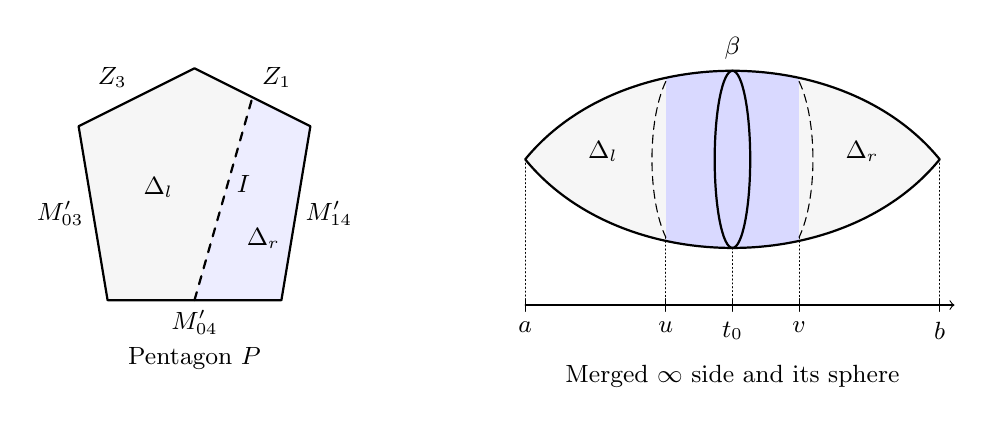
\begin{tikzpicture}[font=\small,line cap=round,line join=round]
  \begin{scope}[xshift=2.4cm,yshift=1.9cm,scale=.92]
    \coordinate (a) at (-1.6,1);
    \coordinate (b) at (0,1.8);
    \coordinate (c) at (1.6,1);
    \coordinate (d) at (1.2,-1.4);
    \coordinate (e) at (-1.2,-1.4);
    \coordinate (istart) at (0,-1.4);
    \coordinate (iend) at (.8,1.4);
    \fill[gray!7] (a)--(b)--(iend)--(istart)--(e)--cycle;
    \fill[blue!7] (iend)--(c)--(d)--(istart)--cycle;
    \draw[thick] (a)--(b)--(c)--(d)--(e)--cycle;
    \draw[thick,dashed] (istart)--(iend);
    \node[right] at (.45,.2) {$I$};
    \node at (-.5,.15) {$\Delta_l$};
    \node at (.95,-.55) {$\Delta_r$};
    \node[above left] at (-.8,1.4) {$Z_3$};
    \node[above right] at (.8,1.4) {$Z_1$};
    \node[left] at (-1.4,-.2) {$M_{03}'$};
    \node[right] at (1.4,-.2) {$M_{14}'$};
    \node[below] at (0,-1.4) {$M_{04}'$};
    \node at (0,-2.2) {Pentagon $P$};
  \end{scope}
  \begin{scope}[xshift=6.6cm,yshift=2.4cm,xscale=.94]
    \begin{scope}
      \clip (0,0) .. controls (1.3,1.5) and (4.3,1.5) .. (5.6,0)
        .. controls (4.3,-1.5) and (1.3,-1.5) .. cycle;
      \fill[gray!7] (0,-1.6) rectangle (5.6,1.6);
      \fill[blue!15] (1.9,-1.6) rectangle (3.7,1.6);
    \end{scope}
    \draw[thick] (0,0) .. controls (1.3,1.5) and (4.3,1.5) .. (5.6,0)
      .. controls (4.3,-1.5) and (1.3,-1.5) .. cycle;
    \draw[densely dashed] (1.9,.99) .. controls (1.65,.5) and (1.65,-.5) .. (1.9,-.99);
    \draw[densely dashed] (3.7,.99) .. controls (3.95,.5) and (3.95,-.5) .. (3.7,-.99);
    \draw[thick] (2.8,0) ellipse [x radius=.24,y radius=1.125];
    \node at (1.05,.1) {$\Delta_l$};
    \node at (4.55,.1) {$\Delta_r$};
    \node[above] at (2.8,1.15) {$\beta$};
    \draw[thin,->] (0,-1.85)--(5.8,-1.85);
    \foreach \x/\name in {0/a,1.9/u,2.8/t_0,3.7/v,5.6/b} {
      \draw (\x,-1.77)--(\x,-1.93);
      \node[below] at (\x,-1.94) {$\name$};
    }
    \draw[densely dotted] (0,0)--(0,-1.75);
    \draw[densely dotted] (1.9,-.99)--(1.9,-1.75);
    \draw[densely dotted] (2.8,-1.125)--(2.8,-1.75);
    \draw[densely dotted] (3.7,-.99)--(3.7,-1.75);
    \draw[densely dotted] (5.6,0)--(5.6,-1.75);
    \node at (2.8,-2.75) {Merged $\infty$ side and its sphere};
  \end{scope}
\end{tikzpicture}

\caption{The two contractions of the pentagon loop test.
Left: the interval $I$ separates the incompatible ball edges
$M_{03}'$ and $M_{14}'$; each region uses the disk lying in its ball cap.
Right: the inverse image of the merged $\infty$ side $[a,b]$ is a
sphere.  The circle over $t_0$ is $\beta$, and the preimages of
$[a,t_0]$ and $[t_0,b]$ are $\Delta_l$ and $\Delta_r$.
The shaded annulus is the part in the inserted $D$ piece.
Concatenating the disk contractions gives a sweep of $\pm S$.
The drawing is schematic, and the $D$ neck remains finite.}
\label{fig:negative:contraction}
\end{figure}

We check its compactification uniformly before using its boundary
formula.  At a primary edge, the unconstrained equation projection
has at most one parameter and is excluded by the central cost.
The contraction mark cannot remedy an empty equation projection.
At a true central end the extra irreducible trajectory gives cost
at least $4-p>1$ for $p\le2$ \emph{equation} parameters, again
independent of the mark.  Positive cap or neck loss and bubbles obey
the same inequalities as in Lemma~\ref{lem:negative:pentagon}.
At $M_{04}'$, $M_{03}'$, or $M_{14}'$ a zero-charge cap misses the
test because the chosen contraction lies in that simply connected
cap.  The collapsed end is also uniformly disjoint from the cut.

The latter avoidance is valid even while the hidden $D$ neck becomes
arbitrarily long.  The sphere meets $D=S^1\times D^3$ in $S^1$
times a diameter of $D^3$.  In each stretched collar its intersection
is consequently $S^1$ times a pole of $S^2$ times the neck interval.
The contractions can therefore be taken along the merged side, using
at each mark a free-circle loop in one slice of the neck or in one
of the two bodies, with uniformly bounded spatial length and
derivatives.  Central holonomy requires no comparison
of frames transported down the neck.  Suppose uniform avoidance
failed for arbitrarily small part perturbations.  Ideal compactness
and the charge exclusions just proved would give matching flat
data on a zero-charge cap and its neck pieces.  These glue to a
flat on the whole simply connected cap, and the root from $W'$
normalizes it absolutely.  A mark remaining on a body then has
holonomy tending to $+\id$.  For a mark escaping along the middle,
Lemma~\ref{lem:ordinary:neck-decay} gives the same conclusion:
normal modes decay and the harmonic slice remains in the matching
flat orbit.  Both conclusions contradict the value $-\id$.
The argument works also at nested compatible corners, using the
innermost required cap.  Thus first choose the sufficiently small
limiting part perturbations with this avoidance, and only then the
large finite $D$ neck.  This order also permits the small generic
cut perturbations needed for regularity.

Apply the one-dimensional mod-two boundary formula on the two
regions.  Their original pentagon contributions add to the original
count; the collapsed ends and the exterior parameter edges contribute
nothing.  True irreducible end breaks give a chain homotopy.  The
remaining boundary lies on $I$, where the two disk contractions
concatenate to a sweep of their union sphere.  Its dimension is
\[
 i'+\underbrace{1}_{I}+\underbrace{1}_{s}-3=0.
\]
This is exactly the interval count with $x(S)$, up to reversal of
the sweep and the fixed tensor identifications.  Reversal is
irrelevant modulo two.

Finally this induced interval data may be made identical to the
chosen data for $B$.  Keep the exterior at $M_{04}'$ fixed and common
for the two lifts.  At index one there are no solutions near that
endpoint: a nonflat cap costs at least two with no exterior
parameters, and a flat cap misses the sweep.  Hence tensor-paired
cap regularizations and cut data may be inserted there, stationary
at the endpoint, without changing the count.  Subsequent comparisons
are precisely the compatible homotopies in
Proposition~\ref{prop:negative:invariance}.  This proves the lemma.
\end{proof}

\begin{proof}[Proof of Theorem~\ref{thm:negative:unit}]
Propositions~\ref{prop:negative:local-sign} and
\ref{prop:negative:invariance} give the integral chain map, its
homotopy invariance, and its coherent local sign convention.
Lemma~\ref{lem:negative:four-topology} identifies the $Z_2$ face
with a product of ordinary mod-two units.
Lemma~\ref{lem:negative:faces} and the associahedron boundary formula
identify that product on homology with the surviving pentagon count.
Lemmas~\ref{lem:negative:pentagon} and \ref{lem:negative:sweeps}
identify the latter with $B$ modulo two.  Thus $B$ induces an
isomorphism, as asserted.
\end{proof}
